\documentclass[tikz,border=5pt]{standalone}
\usepackage{amsmath,amssymb}
\usetikzlibrary{arrows.meta,positioning,decorations.pathmorphing}
\begin{document}
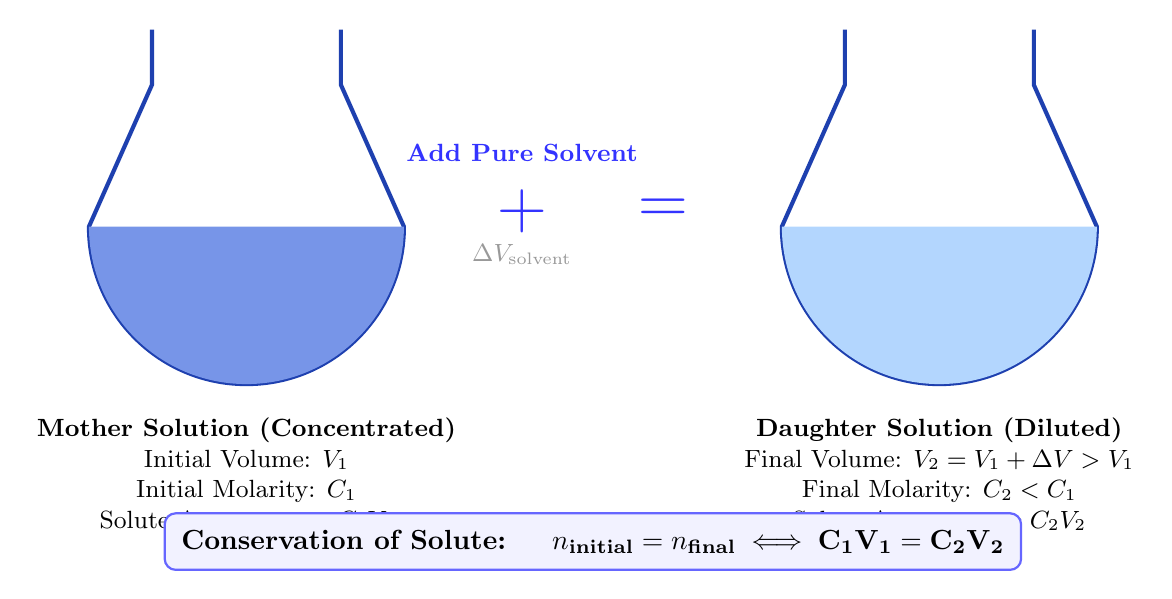
\begin{tikzpicture}[>=Stealth, font=\sffamily, thick]
  \definecolor{flaskblue}{HTML}{1E40AF}
  \definecolor{solutedark}{HTML}{1D4ED8}
  \definecolor{solutelight}{HTML}{93C5FD}

  % Mother solution
  \begin{scope}[shift={(0,0)}]
    \draw[line width=1.5pt, flaskblue] (-1.2,2.5) -- (-1.2,1.8) -- (-2,0) arc[start angle=180, end angle=360, radius=2] -- (1.2,1.8) -- (1.2,2.5);
    \clip (-2,0) arc[start angle=180, end angle=360, radius=2] -- (2,0) -- (-2,0);
    \fill[solutedark!60] (-2.2,-2.2) rectangle (2.2,0.3);
  \end{scope}
  \node[anchor=north, align=center, font=\small] at (0,-2.3) {
    \textbf{Mother Solution (Concentrated)}\\
    Initial Volume: $V_1$\\
    Initial Molarity: $C_1$\\
    Solute Amount: $n = C_1 V_1$
  };

  % Plus solvent
  \node[font=\Huge\bfseries, text=blue!80] at (3.5,0.2) {$+$};
  \node[anchor=south, font=\bfseries\small, text=blue!80] at (3.5,0.7) {Add Pure Solvent};
  \node[anchor=north, font=\small, text=gray!80] at (3.5,-0.1) {$\Delta V_{\text{solvent}}$};

  % Equals
  \node[font=\Huge\bfseries, text=blue!80] at (5.3,0.2) {$=$};

  % Daughter solution
  \begin{scope}[shift={(8.8,0)}]
    \draw[line width=1.5pt, flaskblue] (-1.2,2.5) -- (-1.2,1.8) -- (-2,0) arc[start angle=180, end angle=360, radius=2] -- (1.2,1.8) -- (1.2,2.5);
    \clip (-2,0) arc[start angle=180, end angle=360, radius=2] -- (2,0) -- (-2,0);
    \fill[solutelight!70] (-2.2,-2.2) rectangle (2.2,1.4);
  \end{scope}
  \node[anchor=north, align=center, font=\small] at (8.8,-2.3) {
    \textbf{Daughter Solution (Diluted)}\\
    Final Volume: $V_2 = V_1 + \Delta V > V_1$\\
    Final Molarity: $C_2 < C_1$\\
    Solute Amount: $n = C_2 V_2$
  };

  % Invariant banner
  \node[draw=blue!60, fill=blue!5, rounded corners=4pt, inner sep=6pt, font=\bfseries\normalsize] at (4.4, -4.0) {
    Conservation of Solute: \quad $n_{\text{initial}} = n_{\text{final}} \iff \mathbf{C_1 V_1 = C_2 V_2}$
  };
\end{tikzpicture}
\end{document}
